

The vector equation of a line can be expressed as 
\begin{align}
    \vec{x} = \vec{q} +\mu\vec{m} \label{eq:solutions/4/2/3/vec_eqn_of_line}
\end{align}
The general equation of a second degree can be expressed as :
\begin{align}
\vec{x}^T\vec{V}\vec{x}+2\vec{u}^T\vec{x}+f=0\label{eq:solutions/4/2/3/gen__quad_eqn}
\end{align}


  %  \begin{figure}[!ht]
    %\centering
    %\resizebox{\columnwidth}{!}{\begin{tikzpicture}
\draw (4,4) node[anchor=south]{$A$}
   -- (0,0) node[anchor=north]{$B$}
   -- (4,0) node[anchor=north]{$M$}
   -- (6,0) node[anchor=north]{$D$}
   -- (12,0) node[anchor=north]{$C$}
  -- cycle 
     (4,4) -- (6,0)
     (4,4) -- (4,0);
\end{tikzpicture}}
    %\caption{$\triangle{ABC}$ with $AD$ as median and $AM \perp BC$}
    %\label{eq:solutions/4/2/3/fig:triangle}
   % \end{figure}

Comparing \eqref{eq:solutions/4/2/3/given_circle_eq} with \eqref{eq:solutions/4/2/3/gen__quad_eqn}
\begin{align}
\vec{u}=\myvec{-5 \\ -1}, f=13 
\end{align}
If $\vec{n}$ is the normal vector of a line, equation of that line can be written as 
\begin{align}
\vec{n}^T\vec{x} = c \label{eq:solutions/4/2/3/eq1}
\end{align}
Comparing \eqref{eq:solutions/4/2/3/given_line_eq} with \eqref{eq:solutions/4/2/3/eq1}
\begin{align}
\vec{n} = \myvec{3 \\ 2}\label{eq:solutions/4/2/3/eq2}
\end{align}
 The point of contact $\vec{q}$, of a line with a normal vector $\vec{n}$ to the conic in \eqref{eq:solutions/4/2/3/gen__quad_eqn} is given by:
\begin{align}
\vec{q} = \vec{V}^{-1}\brak{\kappa \vec{n}-\vec{u}} 
%\label{eq:solutions/4/2/3/eq3} 
\\
\kappa = \pm \sqrt{\frac{\vec{u}^T\vec{V}^{-1}\vec{u}-f}{\vec{n}^T\vec{V}^{-1}\vec{n}}} \label{eq:solutions/4/2/3/eq4}
\end{align}
We know that, for a circle, 
\begin{align}
\vec{V} = \vec{I}  
\end{align}
and from the properties of an Identity matrix, 
\begin{align}
\vec{I}^{-1} &= \vec{I} \\
\vec{I}\vec{X} &= \vec{X}   
\end{align}
Solving for the point of contact using the above equations we get,
\begin{align}
\kappa &= \pm \sqrt{\frac{\myvec{ -5 & -1 }\myvec{-5 \\ -1} - 13}{\myvec{3 & 2 }\myvec{3 \\ 2 }}} \\
&= \pm \sqrt{\frac{26 - 13}{13}} \\
& =  \pm \sqrt{1} \\
q &= \myvec{3 \\2 } - \myvec{-5 \\ -1} \\
&= \myvec{8 \\ 3}
\end{align}
If the line in \eqref{eq:solutions/4/2/3/vec_eqn_of_line} touches  \eqref{eq:solutions/4/2/3/gen__quad_eqn} at exactly one point $\vec{q}$, then 
\begin{align}
\vec{m}^T\brak{\vec{V}\vec{q}+\vec{u}} = 0 \label{eq:solutions/4/2/3/eq3}
\end{align}
It can seen that for the given line
\begin{align}
\vec{m} = \myvec{1 \\ -1.5} 
\end{align}
Solving \eqref{eq:solutions/4/2/3/eq3} for given line and circle, we get
\begin{align}
&= \myvec{1 & -1.5}\brak{\myvec{8 \\ 3}+\myvec{-5 \\ -1}} \\
&= \myvec{1 & -1.5}\myvec{3 \\ 2}\\
&= 0
\end{align}
Hence, it is proved that the given line touches the given circle at only one point and so it is a tangent.
\begin{figure}[!ht]
\centering
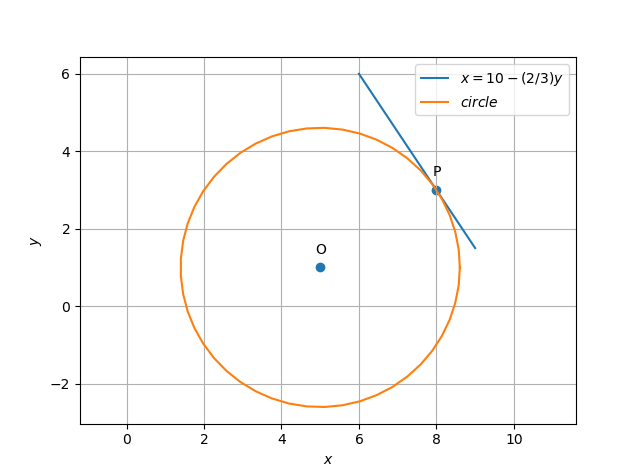
\includegraphics[width=\columnwidth]{./solutions/4/2/3/assignment_5_fig.png}
\caption{Circle with center (5 1) and having the line (3 2)x =30 as tangent with (8 3) as point of contact.}
\label{eq:solutions/4/2/3/Fig:Circle}
\end{figure}
